\documentclass{beamer}
\usepackage[english, russian]{babel}
\usepackage[T2A]{fontenc}
\usepackage[utf8]{inputenc}
\usepackage{indentfirst}
\usepackage{amsmath, amsfonts, amssymb, amsthm, mathtools}
\usepackage[export]{adjustbox}
\usepackage{graphicx} 
\graphicspath{ {./images/} }

\usepackage{subcaption}
\usepackage{verbatim}

\usepackage{minted}{\setlength{\parskip}{0pt}}

\usepackage{hyperref}

\hypersetup{
    colorlinks=true,
    linkcolor=blue,
    filecolor=magenta,      
    urlcolor=black,
    pdftitle={Overleaf Example},
    pdfpagemode=FullScreen,
    }


\title{Отчет по лабораторной работе № 16. \\ Базовая защита от атак типа "brute force"}
\author{Данила Стариков \\ НПИбд-02-22}
\date{2024}

\begin{document}

\maketitle
\newpage

\tableofcontents

\newpage
\section{Цель работы}
Получить навыки работы с программным средством Fail2ban для обеспечения базовой защиты от атак типа "brute force".

\newpage
\section{Выполнение работы}
\subsection{Защита с помощью Fail2ban}

\begin{enumerate}
\item На сервере установили {\tt fail2ban}:
\begin{minted}{bash}
    dnf -y install fail2ban
\end{minted}

\item Запустили сервис {\tt fail2ban} (Рис. \ref{01}):
\begin{minted}{bash}
    systemctl start fail2ban
    systemctl enable fail2ban
\end{minted}

  \begin{center}
    \centering
    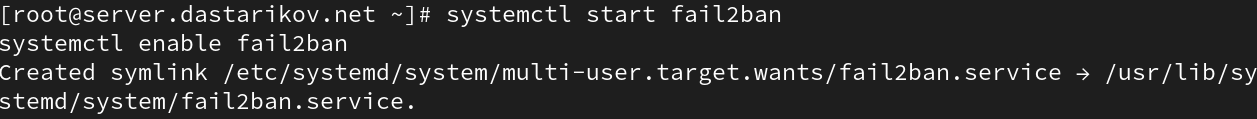
\includegraphics[width=\textwidth]{../images/image01.png}
    \captionof{figure}{Запуск сервиса \texttt{fail2ban}.}
    \label{01}
  \end{center}

\item В дополнительном терминале запустили просмотр журнала событий {\tt fail2ban} (Рис. \ref{02}):
\begin{minted}{bash}
    tail -f /var/log/fail2ban.log
\end{minted}

  \begin{center}
    \centering
    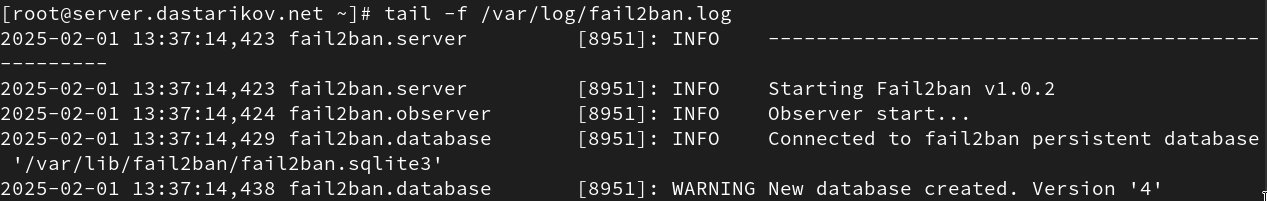
\includegraphics[width=\textwidth]{../images/image02.png}
    \captionof{figure}{Просмотр журнала событий \texttt{fail2ban}.}
    \label{02}
  \end{center}

\item Создали файл с новой конфигурацией {\tt fail2ban}:
\begin{minted}{bash}
    touch /etc/fail2ban/jail.d/customisation.local
\end{minted}

\item В файле {\tt /etc/fail2ban/jail.d/customisation.local}:
  \begin{itemize}
  \item задали время блокирования на 1 час (время задаётся в секундах):
\begin{minted}{bash}
      [DEFAULT]
      bantime = 3600
\end{minted}

  \item включили защиту SSH:
\begin{minted}{bash}
      [sshd]
      port = ssh,2022
      enabled = true

      [sshd-dos]
      filter = sshd
      enabled = true

      [selinux-ssh]
      enabled = true
\end{minted}
  \end{itemize}

\item Перезапустили {\tt fail2ban}:
\begin{minted}{bash}
    systemctl restart fail2ban
\end{minted}

\item Просмотрели журналы событий (Рис. \ref{03}):
\begin{minted}{bash}
    tail -f /var/log/fail2ban.log
\end{minted}


  \begin{center}
    \centering
    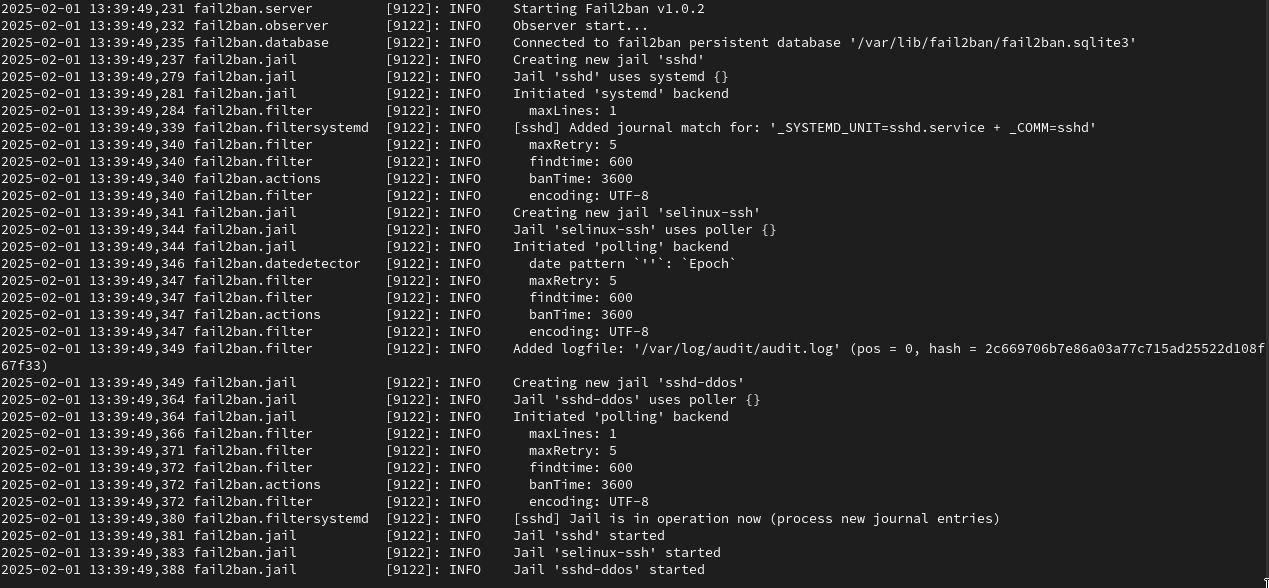
\includegraphics[width=\textwidth]{../images/image03.png}
    \captionof{figure}{Просмотр журнала событий после первоначальной настройки \texttt{fail2ban}.}
    \label{03}
  \end{center}

\item В файле {\tt /etc/fail2ban/jail.d/customisation.local} включите защиту HTTP:
\begin{minted}{bash}
    #
    # HTTP servers
    #

    [apache-auth]
    enabled = true

    [apache-badbots]
    enabled = true

    [apache-noscript]
    enabled = true

    [apache-overflows]
    enabled = true

    [apache-nohome]
    enabled = true

    [apache-botsearch]
    enabled = true

    [apache-fakegooglebot]
    enabled = true

    [apache-modsecurity]
    enabled = true

    [apache-shellshock]
    enabled = true
\end{minted}

\item Перезапустили {\tt fail2ban}
\begin{minted}{bash}
    systemctl restart fail2ban
\end{minted}

\item Посмотрели журнал событий (Рис. \ref{04}-\ref{06}):
\begin{minted}{bash}
    tail -f /var/log/fail2ban.log
\end{minted}

  \begin{center}
    \centering
    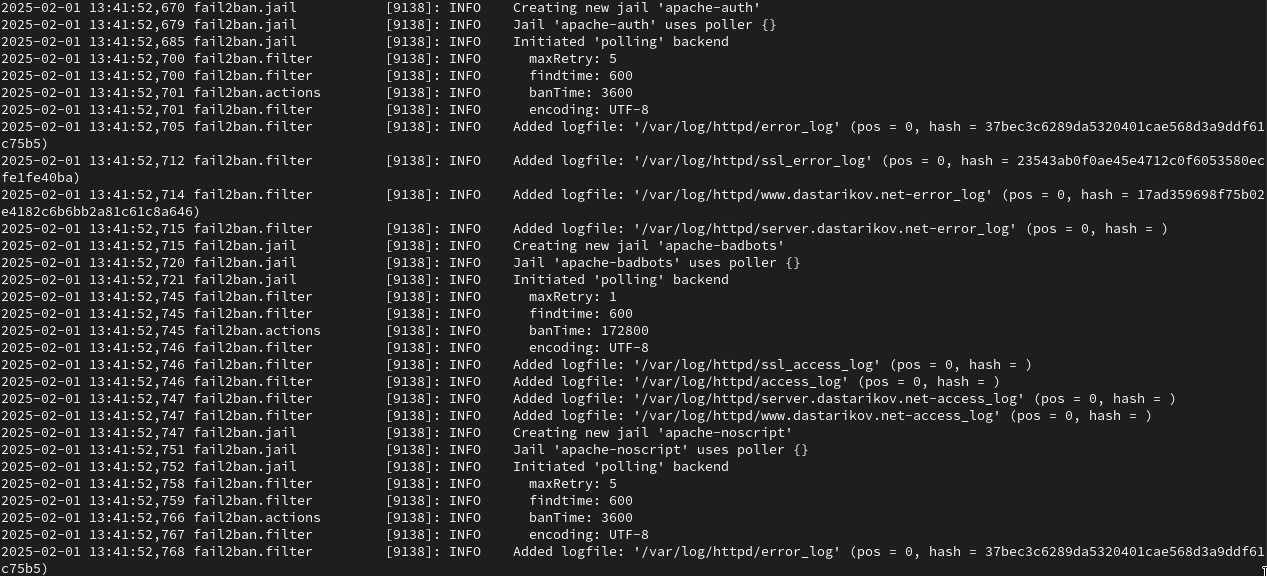
\includegraphics[width=\textwidth]{../images/image04.png}
    \captionof{figure}{Логи, связанные с защитой HTTP (Часть 1).}
    \label{04}
  \end{center}

  \begin{center}
    \centering
    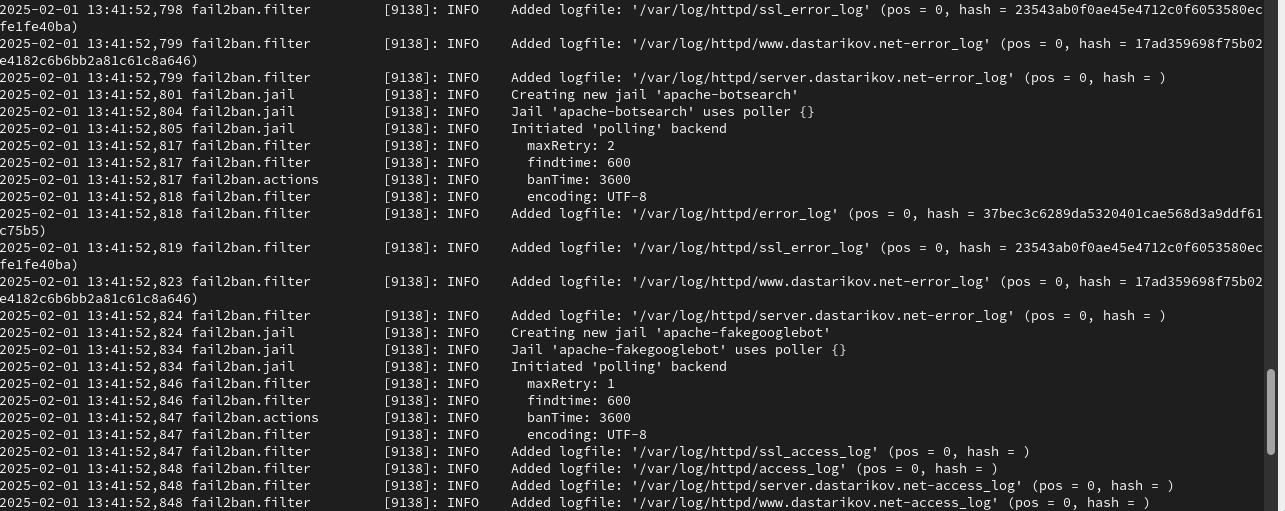
\includegraphics[width=\textwidth]{../images/image05.png}
    \captionof{figure}{Логи, связанные с защитой HTTP (Часть 2).}
    \label{05}
  \end{center}

  \begin{center}
    \centering
    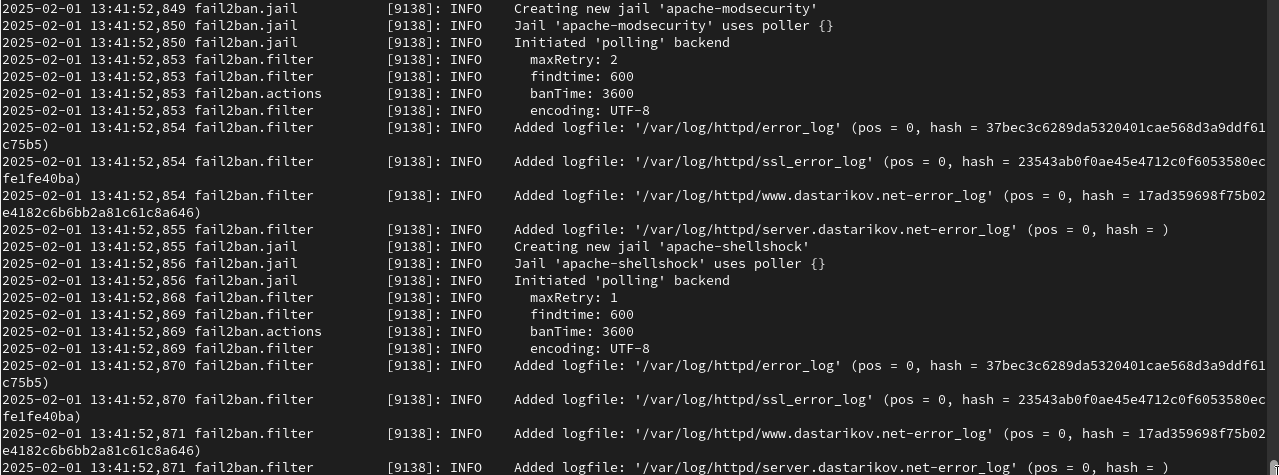
\includegraphics[width=\textwidth]{../images/image06.png}
    \captionof{figure}{Логи, связанные с защитой HTTP (Часть 3).}
    \label{06}
  \end{center}

\item В файле {\tt /etc/fail2ban/jail.d/customisation.local} включите защиту почты:
\begin{minted}{bash}
    #
    # Mail servers
    #

    [postfix]
    enabled = true

    [postfix-rbl]
    enabled = true

    [dovecot]
    enabled = true

    [postfix-sasl]
    enabled = true
\end{minted}

\item Перезапустили {\tt fail2ban}:
\begin{minted}{bash}
    systemctl restart fail2ban
\end{minted}

\item Посмотрели журнал событий (Рис. \ref{08}):
\begin{minted}{bash}
    tail -f /var/log/fail2ban.log
\end{minted}
\end{enumerate}


\begin{center}
  \centering
  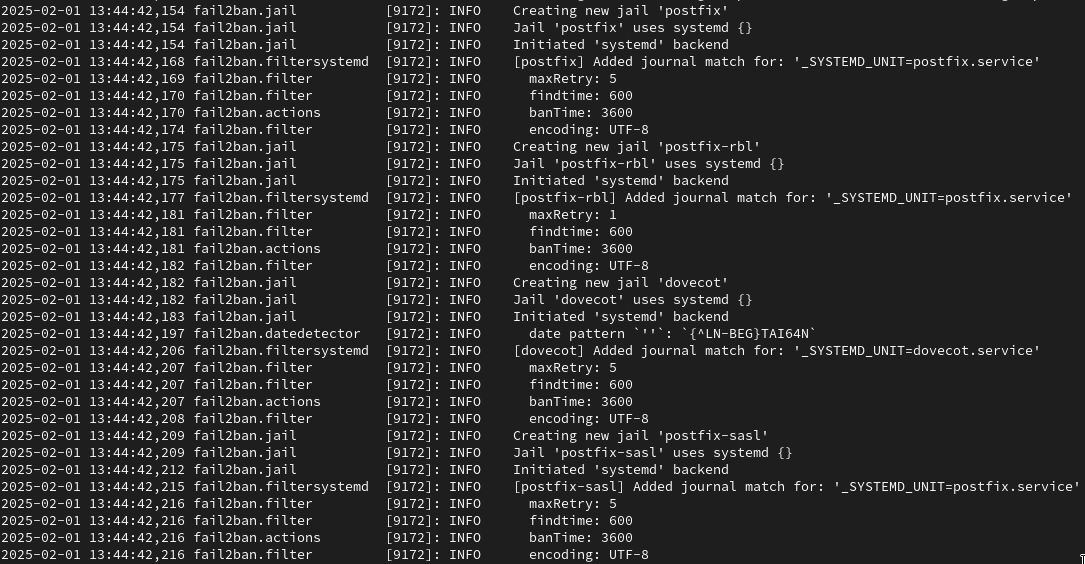
\includegraphics[width=\textwidth]{../images/image08.png}
  \captionof{figure}{Логи, связанные с защитой почты.}
  \label{08}
\end{center}

\subsection{Проверка работы Fail2ban}

\begin{enumerate}
\item На сервере посмотрели статус {\tt fail2ban} (Рис. \ref{09}):
\begin{minted}{bash}
    fail2ban-client status
\end{minted}

  \begin{center}
    \centering
    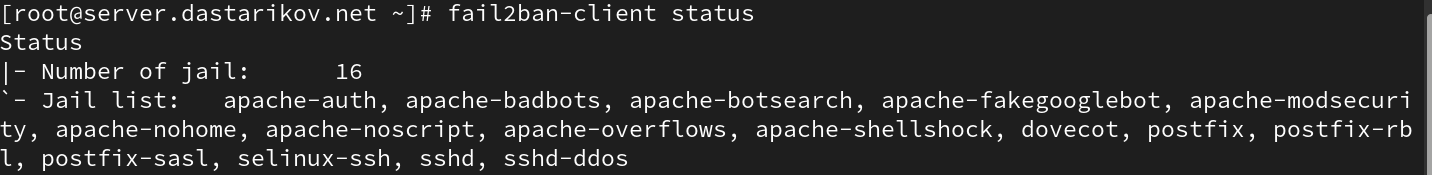
\includegraphics[width=\textwidth]{../images/image09.png}
    \captionof{figure}{Просмотр статуса \texttt{fail2ban}.}
    \label{09}
  \end{center}

\item Посмотрели статус защиты SSH и {\tt fail2ban} (Рис. \ref{10}):
\begin{minted}{bash}
    fail2ban-client status sshd
\end{minted}

  \begin{center}
    \centering
    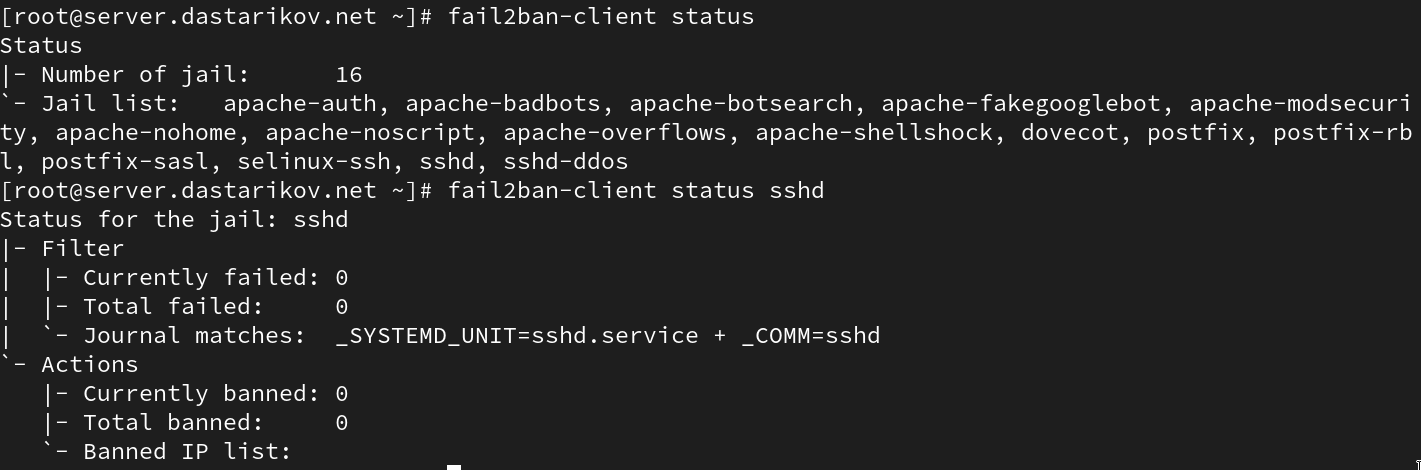
\includegraphics[width=\textwidth]{../images/image10.png}
    \captionof{figure}{Просмотр статуса защиты SSH.}
    \label{10}
  \end{center}

\item Установили максимальное количество ошибок для SSH, равное 2 (Рис. \ref{11}):
\begin{minted}{bash}
    fail2ban-client set sshd maxretry 2
\end{minted}

  \begin{center}
    \centering
    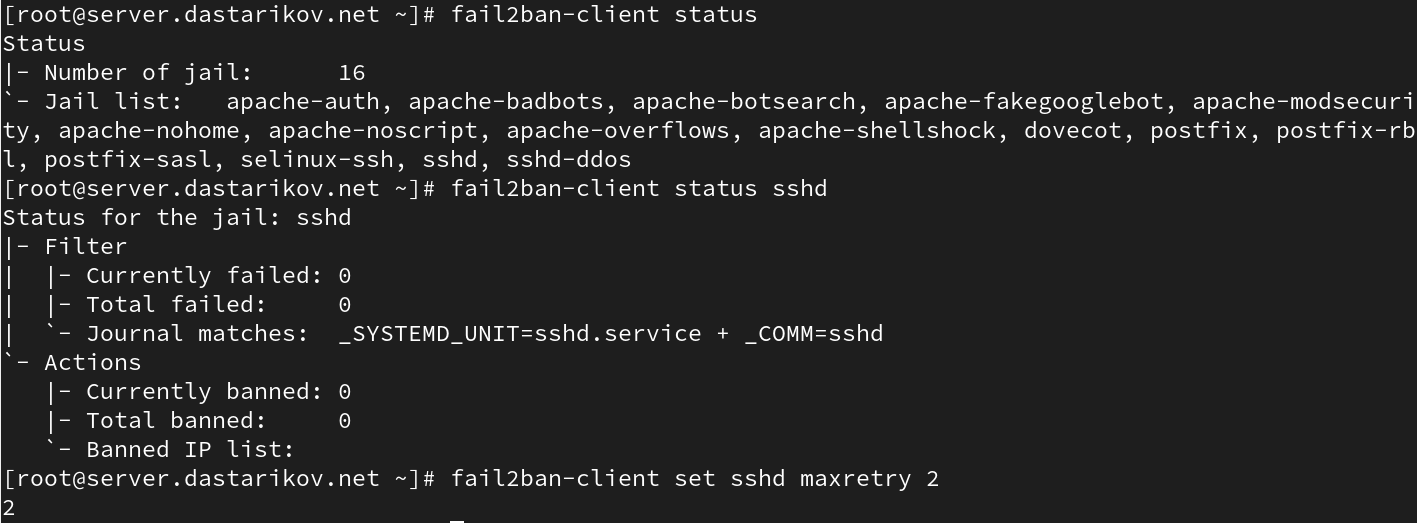
\includegraphics[width=\textwidth]{../images/image11.png}
    \captionof{figure}{Установка максимального количества ошибок для SSH.}
    \label{11}
  \end{center}

\item С клиента попытались зайти по SSH на сервер с неправильным паролем (Рис. \ref{12}).

  \begin{center}
    \centering
    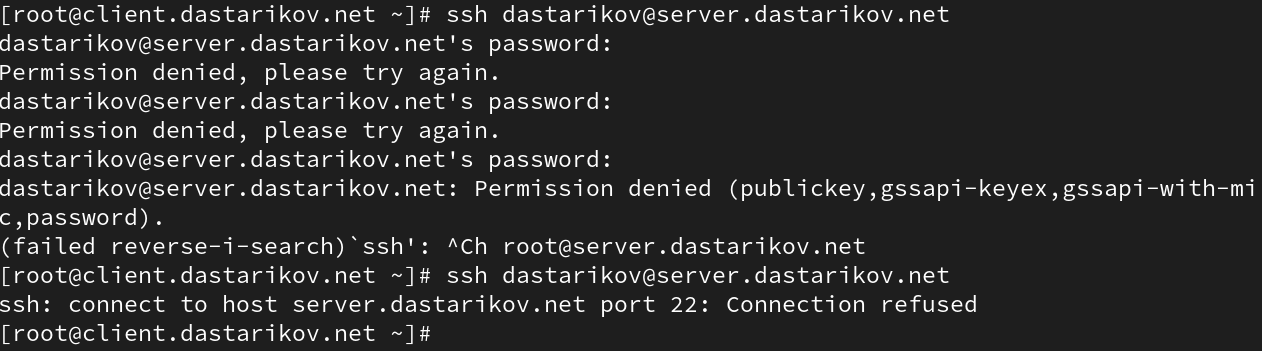
\includegraphics[width=\textwidth]{../images/image12.png}
    \captionof{figure}{Попытка зайти на сервер через SSH с неправильным паролем.}
    \label{12}
  \end{center}

\item На сервере посмотрели статус SSH (Рис. \ref{13}):
\begin{minted}{bash}
    fail2ban-client status sshd
\end{minted}

\item Убедились, что произошла блокировка адреса клиента (Рис. \ref{13}).

  \begin{center}
    \centering
    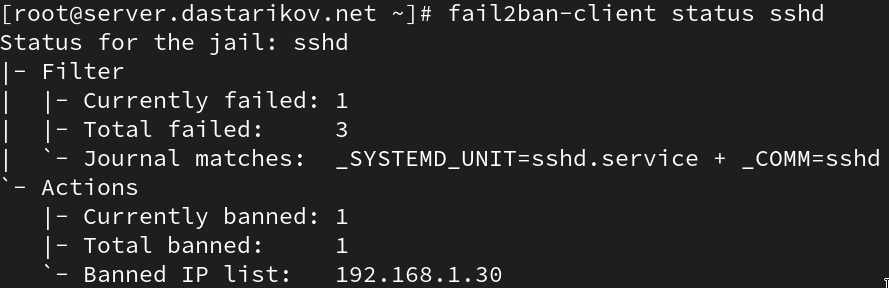
\includegraphics[width=\textwidth]{../images/image13.png}
    \captionof{figure}{Просмотр статуса защиты SSH.}
    \label{13}
  \end{center}

\item Разблокировали IP-адрес клиента (Рис. \ref{14}):
\begin{minted}{bash}
    fail2ban-client set sshd unbanip 192.168.1.30
\end{minted}

\item Вновь посмотрели статус защиты SSH (Рис. \ref{14}):
\begin{minted}{bash}
    fail2ban-client status sshd
\end{minted}

  \begin{center}
    \centering
    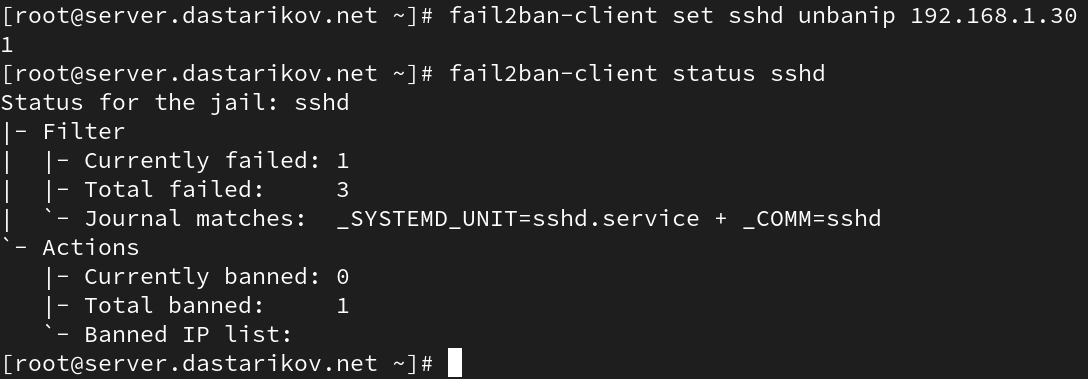
\includegraphics[width=\textwidth]{../images/image14.png}
    \captionof{figure}{Разблокировка ip-адреса клиента.}
    \label{14}
  \end{center}

  Убедились, что блокировка клиента снята.

  \begin{center}
    \centering
    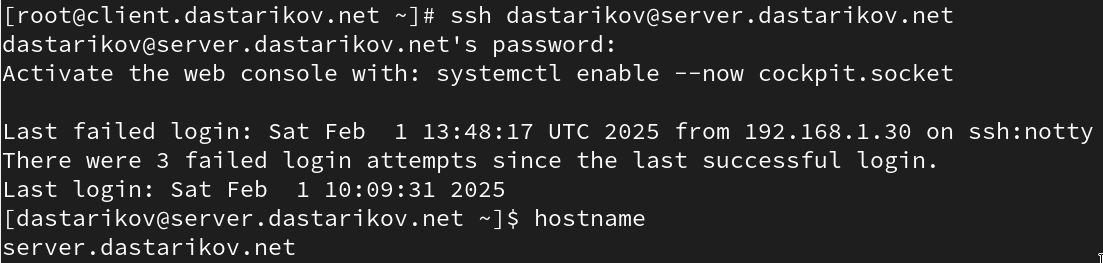
\includegraphics[width=\textwidth]{../images/image15.png}
    \captionof{figure}{Проверка снятия блокировки.}
    \label{15}
  \end{center}

\item На сервере внесли изменение в конфигурационный файл {\tt /etc/fail2ban/jail.d/customisation.local}, добавив в раздел по умолчанию игнорирование адреса клиента
\begin{minted}{bash}
    [DEFAULT]
    bantime = 3600

    ingoreip = 127.0.0.1/8 192.168.1.30
\end{minted}

\item Перезапустили {\tt fail2ban}.
\item Посмотрели журнал событий (Рис. \ref{19}):
\begin{minted}{bash}
    tail -f /var/log/fail2ban.log
\end{minted}

  \begin{center}
    \centering
    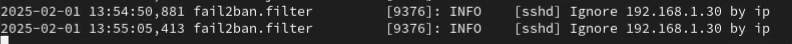
\includegraphics[width=\textwidth]{../images/image19.png}
    \captionof{figure}{Логи журнала об игнорировании адреса клиента.}
    \label{19}
  \end{center}

\item Вновь попытались войти с клиента на сервер с неправильным паролем (Рис. \ref{16}) и посмотрели статус защиты SSH (Рис. \ref{17}).

  \begin{center}
    \centering
    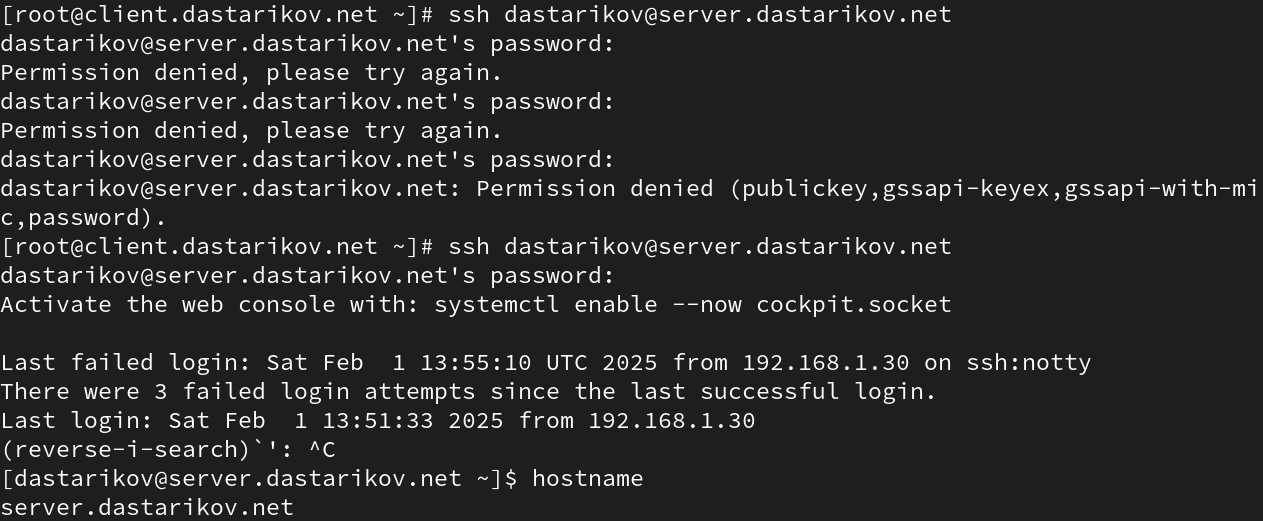
\includegraphics[width=\textwidth]{../images/image16.png}
    \captionof{figure}{Демонстрация игнорирования безуспешных попыток подключения по SSH.}
    \label{16}
  \end{center}

  \begin{center}
    \centering
    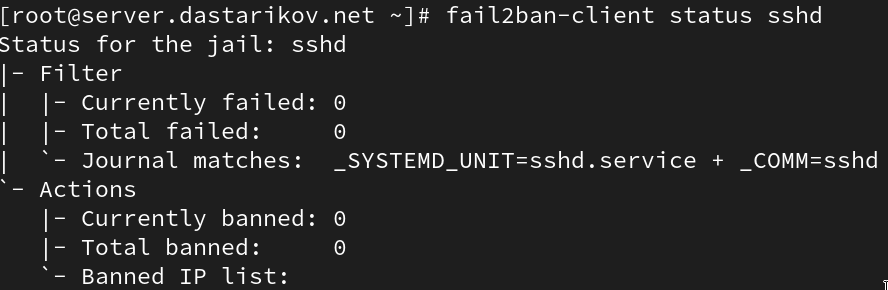
\includegraphics[width=\textwidth]{../images/image17.png}
    \captionof{figure}{Просмотр информации о защите SSH.}
    \label{17}
  \end{center}

\end{enumerate}
\subsection{Внесение изменений в настройки внутреннего окружения виртуальных машин}

\begin{enumerate}
\item На виртуальной машине server перешли в каталог для внесения изменений в настройки внутреннего окружения {\tt /vagrant/provision/server/}, создали в нём каталог {\tt protect}, в который поместили в соответствующие подкаталоги конфигурационные файлы (Рис. \ref{18}):
\begin{minted}{bash}
    cd /vagrant/provision/server
    mkdir -p /vagrant/provision/server/protect/etc/fail2ban/jail.d
    cp -R /etc/fail2ban/jail.d/customisation.local /vagrant/provision/server/protect/etc/fail2ban/jail.d/
\end{minted}

\item В терминале {\tt /vagrant/provision/server} создали исполняемый файл {\tt protect.sh} (Рис. \ref{18}):

\begin{minted}{bash}
    cd /vagrant/provision/server
    touch protect.sh
    chmod +x protect.sh
\end{minted}


  \begin{center}
    \centering
    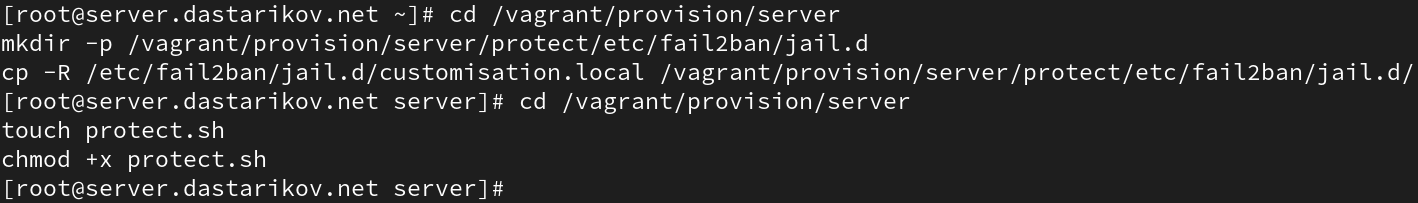
\includegraphics[width=\textwidth]{../images/image18.png}
    \captionof{figure}{Настройка внутреннего окружения сервера.}
    \label{18}
  \end{center}

  Открыли его для редактирования, написали в нём следующий скрипт:

\begin{minted}{bash}
    #!/bin/bash

    echo "Provisioning script $0"

    echo " Install needed packages"
    dnf -y install fail2ban

    echo "Copy configuration files"
    cp -R /vagrant/provision/server/protect/etc/* /etc
    restorecon -vR /etc

    echo "Start fail2ban service"
    systemctl enable fail2ban
    systemctl start fail2ban
\end{minted}

\item Для отработки созданного скрипта во время загрузки виртуальной машины server в конфигурационном файле Vagrantfile добавили в соответствующем разделе конфигураций для сервера:

\begin{minted}{bash}
    server.vm.provision "server protect",
        type: "shell",
        preserve_order: true,
        path: "provision/server/protect.sh"
\end{minted}
\end{enumerate}


\section{Выводы}
Во время выполнения лабораторной работы получили навыки настройки обеспечения базовой защиты от атак типа "brute force" с помощью программы Fail2ban.
\end{document}
